\chapter{Adquisición de datos}

Esta clase tiene como objetivo comprender los pasos básicos para adquirir y procesar imágenes satelitales. Para ello se descargarán imágenes de la web y se procesarán para poder ser utilizadas en el SNAP.

\section{Descarga de imágenes}

Para descargar imágenes utilizaremos el catálogo del \href{https://earthexplorer.usgs.gov/}{Earth Explorer}\footnote{\href{https://earthexplorer.usgs.gov/}{https://earthexplorer.usgs.gov/}}. Para esto debe ingresar a la página y registrarse.


Diríjase a la página y en la pestaña \texttt{Seach Criteria} seleccione \texttt{Address/Place} y escriba \texttt{Iguazú} haciendo luego click en \menu{Show} . Luego haga click sobre el nombre \textt{Misiones Province, Argentina} para seleccionar dicha zona en el mapa (Figura \ref{fig:busqueda}).

\begin{figure}[h!]
    \centering
    %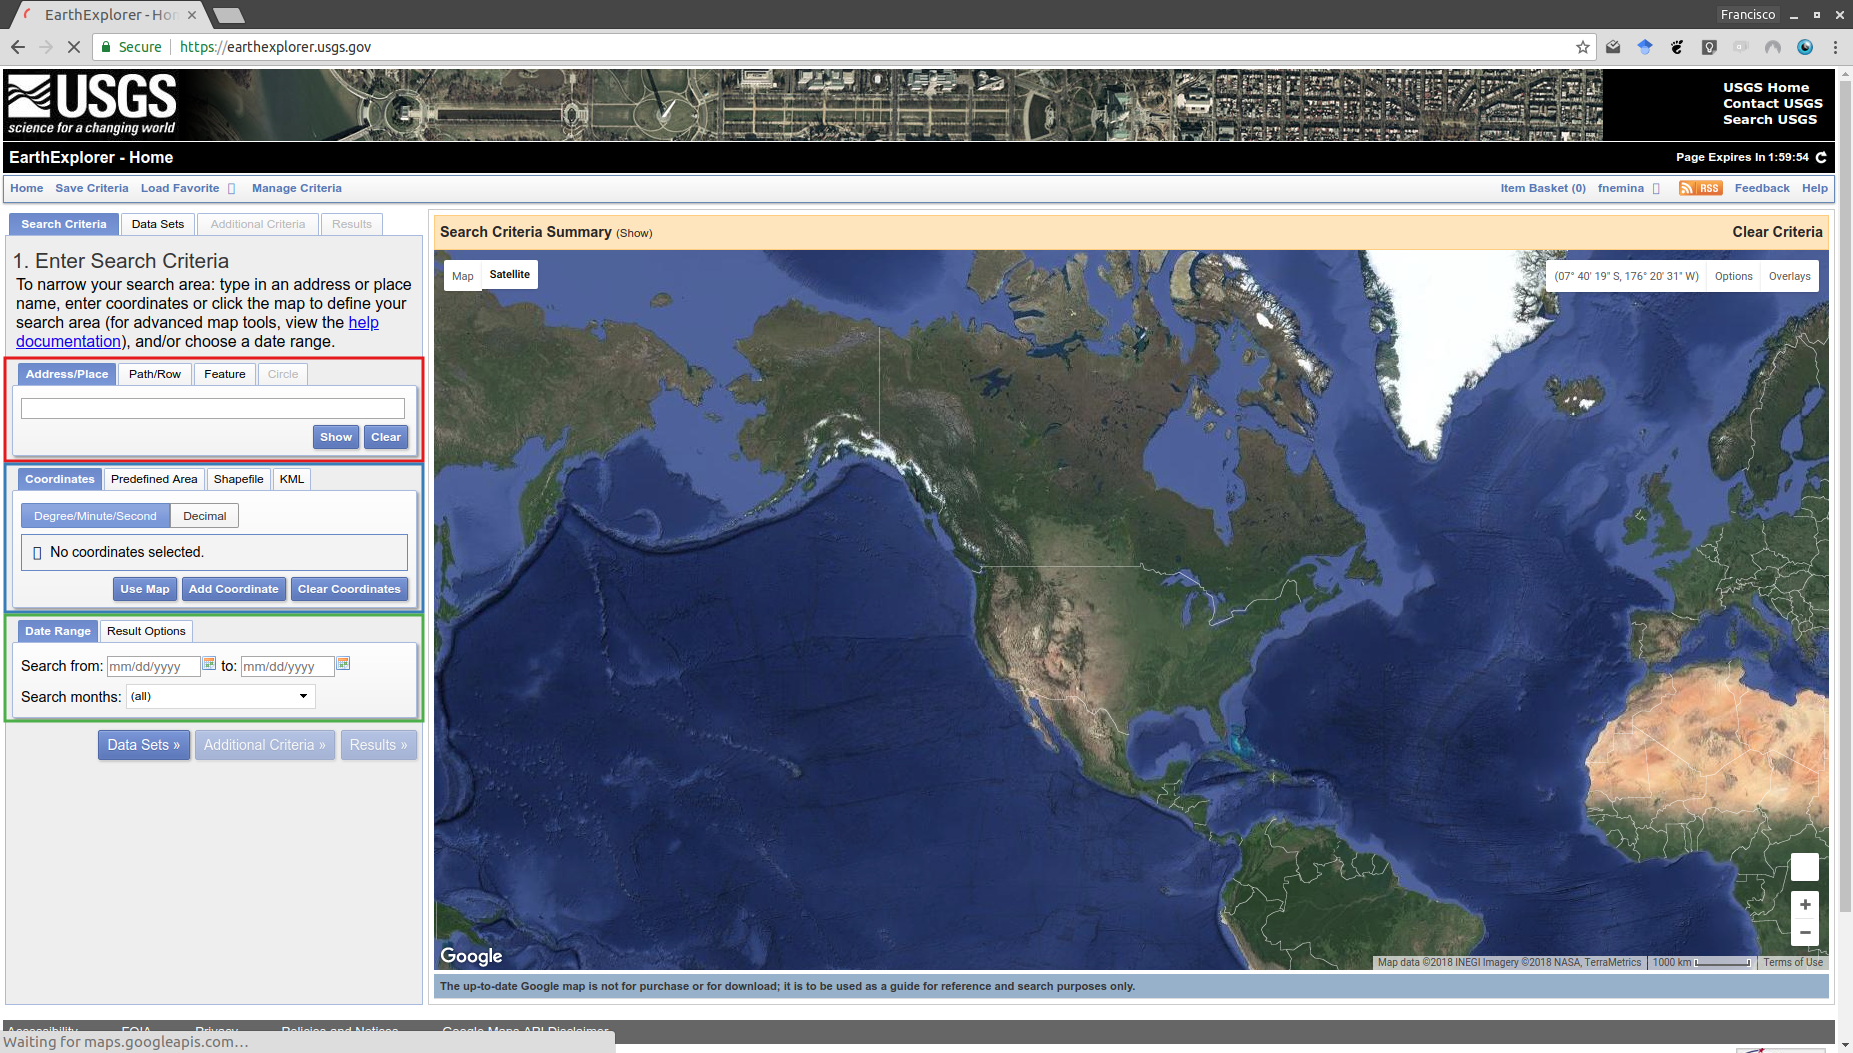
\includegraphics[width=0.7\textwidth]{fig:busqueda.png}
    \caption{Selección de un área de interés en el catálogo \emph{Vertex} del \emph{Alaska Satellite Facility}}
    \label{fig:region}
\end{figure}

Seleccione luego en \menu{Data Range} las fechas 1 de julio de 2017 y 31 de julio de 2017.

\textbf{Observación:} Es posible también dibujar una zona de interés directamente sobre el mapa.
\textbf{Observación:} Para eliminar un punto del mapa haga click en la cruz roja que se encuentra al lado de el en el menú.

Haga click en \menu{Data Sets} y en el cuadro \texttt{Data Set Search:} escriba \texttt{Landsat 8} y seleccione del menú la opción \texttt{Landsat 8 OLI/TIRS C1 Level-2} (Figura \ref{fig:dataset}) para seleccionarlo.

\begin{figure}[h!]
    \centering
    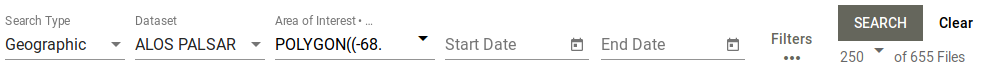
\includegraphics[width=0.7\textwidth]{fig:dataset.png}
    \caption{Selección de \emph{Dataset} en el catálogo \emph{Earth Explorer} del \emph{USGS}.}
    \label{fig:dataset}
\end{figure}

Haga luego click en \menu{Results}.

A la izquierda de la pantalla aparecerá una lista de productos. Busque de ellos el de nombre \emph{LC08_L1TP_224078_20170713_20170726_01_T1
} del 13 de julio del 2017, pertenenciente al path 224 y el row 78. Haga click sobre \menu{Order scene}. (Figura \ref{fig:seleccion})

\begin{figure}[h!]
    \centering
    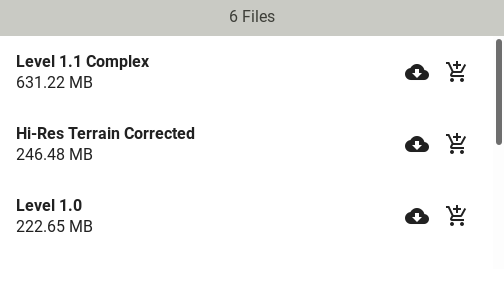
\includegraphics[width=0.7\textwidth]{fig:descarga.png}
    \caption{Selección de producto para la descarga en el catálogo \emph{Vertex} del \emph{USGS}.}
    \label{fig:seleccion}
\end{figure}

Para corroborar el pedido haga click en \menu{View Item Basket} y luego en \menu{Proceed to Checkout}. Finalmente deberá solicitar la imagen haciendo click en \menu{Submit Order}.

El producto descargado pertenece a una serie de producto \emph{on demands} \footnote{A demananda.}. Cuando el mismo esté disponible para descargar se le enviará un correo electrónico notificandolo.

\textbf{Observación:} El tiempo para que el producto esté disponible puede ser de hasta 48 horas.
